\documentclass[10pt]{article}
\usepackage{graphicx}
\usepackage[backend=biber,style=numeric,sorting=ynt]{biblatex}
\usepackage{amsmath, gensymb}

\RequirePackage{array}
\RequirePackage{booktabs} 
\RequirePackage{tabularray} 
\RequirePackage{tabularx} 
\RequirePackage{threeparttable} 
\RequirePackage{tablefootnote} 
\RequirePackage{colortbl} 
\RequirePackage{xcolor}

\addbibresource{references.bib}

\title{Prism Spectrometer} 
\author{Rahmanyaz Annyyev, Hikmat Gulaliyev} 
\date{02 March 2024} 

\begin{document}

\maketitle

\begin{abstract}
In this experiment, we utilize a prism spectrometer---an optical device that separates light into its constituent frequencies---to measure the refractive index of a prism. A collimator with a slit is used to produce a parallel beam of light emitted by a mercury lamp, which is then passed through the prism. The light is then refracted and dispersed into its constituent frequencies. The angle of deviation of the light is measured and used to calculate the refractive index of the prism using a special relation. A graph of the index of refraction versus wavelength is also plotted. The results are compared to the theoretical values and the limitations of the experiment are discussed.
\end{abstract}

\section{Introduction}

The visible spectrum is the portion of electromagnetic radiation that is visible to the human eye. It is composed of light with wavelengths between 380 and 780 nm. Each wavelength, or frequency of light is perceived as a different color by the human eye\cite{Marcus_1998}. Spectrum analysis is the study of measure and interpretation of electromagnetic spectra. It is used in various fields such as physics, chemistry, and astronomy. One of the most important tools in spectrum analysis is the prism spectrometer. 

A prism spectrometer is an optical device, and it is composed of a collimator, a prism, and a telescope. The collimator is a device that produces a parallel beam of light. It is composed of an adjustable slit on one end and a converging lens on the other. The slit is used to control the width of the entering light, and the lens is used to focus the light into a parallel beam. As the beam exits the collimator, it impinges on the prism. The prism rests on a rotatable table, and it is used to refract and disperse the light into its constituent colors. The telescope is used to observe the dispersed light, and it is composed of a lens and an eyepiece. The set of parallel beams of different wavelengths form images of the slit. The telescope can be rotated with the aid of the reticle to position the images for each spectral line. 
The instrument that is used throughout the experiment to measure the angles is called a vernier scale.

In this experiment, we use the spectrometer to measure the refractive index of the prism. The refractive index of a prism is a measure of how much the light is bent as it passes through the prism. Examine Figure~\ref{fig:1}. As you can see, $\delta$ is the angle of deviation of the light---the angle between the incident and emergent beams of light, and $\alpha$ is the apex angle of the prism---the angle between two faces of the prism. The deviation angle is dependent on the wavelength of the light.
\begin{figure}[ht]
    \centering
    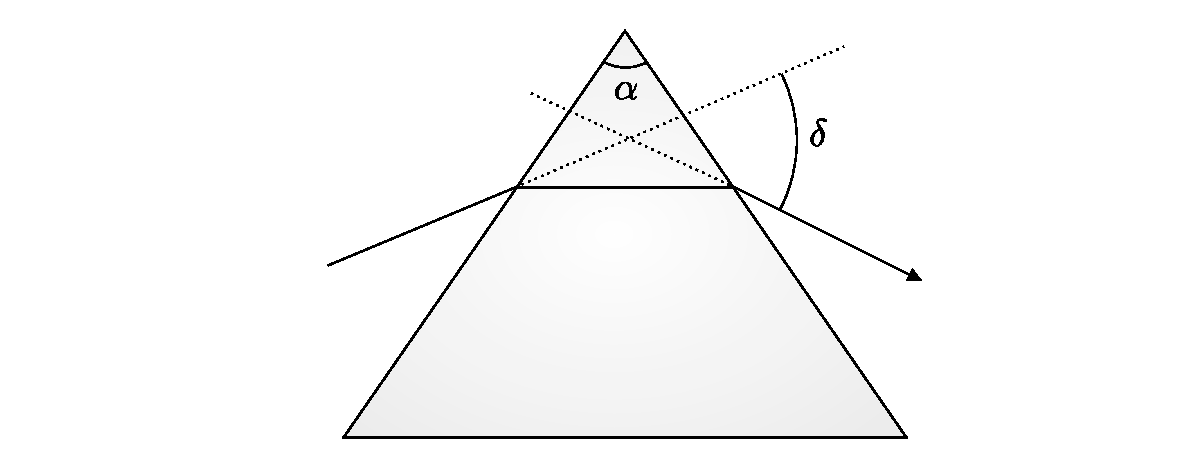
\includegraphics[scale=0.6]{figures/f1.pdf}
    \caption{Refraction of light through a prism.}
    \label{fig:1}
\end{figure}
As we vary the incident angle, the deviation angle changes, and we can obtain its minimum value. This happens when the angle of incidence is equal to the angle of emergence. Hence, in this case, the refractive index of the prism is given by the relation
\begin{equation}
    \label{eq:1}
    n = \frac{\sin\left((\delta_{min}+\alpha) / 2 \right)}{\sin\left(\alpha / 2\right)},
\end{equation}
which is derived from Snell's law,
\begin{equation}
    n_1 \sin(\theta_1) = n_2 \sin(\theta_2),
\end{equation}
where $n_1$ and $n_2$ are the refractive indices of the two media, and $\theta_1$ and $\theta_2$ are the angles of incidence and refraction, respectively. Note that the light is refracted twice as it enters and exits the prism. 

A dispersion curve is a graph of the refractive index versus wavelength. It can be represented using the Cauchy equation,
\begin{equation}
    n(\lambda) = A + \frac{B}{\lambda^2} + \frac{C}{\lambda^4} + \cdots,
\end{equation}
where $A$, $B$, and $C$ are constant pertaining to a specific material. The dispersion curve is used to determine the refractive index of a material at a specific wavelength.

\section{Data \& Results}

The first part of the experiment involved measuring the angle of the prism, $\alpha$. The prism was placed on the rotatable table, and the telescope was used to measure the angle of the prism. The prism was placed in the center of the table, and the telescope was rotated used to measure the angle of the prism. The results are shown in Table~\ref{tab:1}. The average angle of the prism is given by $\bar{\alpha} = 59.87\degree$.

\begin{table}[ht]
    \label{tab:1}
    \centering
    \vspace{4mm}

    \begin{tblr}{
        cells = {halign = c, valign = m},
        row{odd} = {bg = lightgray!5},
        row{1} = {bg = lightgray!20},
        hlines = {},
        vlines = {},
        cell{5}{1}={c=2}{l}
    }
        Position \#1 & Position \#2 & $\alpha_i$ \\
        $52\degree 46'$ & $293\degree 01'$ & $59.86\degree$ \\
        $52\degree 52'$ & $293\degree 05'$ & $59.88\degree$ \\
        $52\degree 48'$ & $293\degree 03'$ & $59.86\degree$ \\
        & & $\bar{\alpha} = 59.87\degree$ \\
    \end{tblr}
    \caption{Data for the prism angle, $\alpha$.}
\end{table}






In this experiment, we employed a mercury lamp as a source of light. 

Calculations for table 2:
\begin{align}
    &\delta_{min}(\text{Violet}) = 360.00\degree-351.80\degree+29.82\degree = 38.02\degree \\
    &\delta_{min}(\text{Blue}) = 360.00\degree-351.80\degree+29.51\degree = 38.31\degree \\
    &\delta_{min}(\text{Green}) = 360.00\degree-351.80\degree+27.63\degree = 40.19\degree \\
    &\delta_{min}(\text{Orange}) = 360.00\degree-351.80\degree+28.64\degree = 39.18\degree 
\end{align}

And the refractive index is given by
\begin{equation}
    n = \frac{\sin\left(\frac{\delta_{min}+\alpha}{2}\right)}{\sin\left(\frac{\alpha}{2}\right)},
\end{equation}
where $\alpha$ is the angle of the prism. Hence, the refractive index for each wavelength is given by
\begin{align}
    n_{\text{Violet}} &= \frac{\sin\left(\frac{38.02\degree+59.87\degree}{2}\right)}{\sin\left(\frac{59.87\degree}{2}\right)} = 1.77 \\
    n_{\text{Blue}} &= \frac{\sin\left(\frac{38.31\degree+59.87\degree}{2}\right)}{\sin\left(\frac{59.87\degree}{2}\right)} = 1.78 \\
    n_{\text{Green}} &= \frac{\sin\left(\frac{40.19\degree+59.87\degree}{2}\right)}{\sin\left(\frac{59.87\degree}{2}\right)} = 1.79 \\
    n_{\text{Orange}} &= \frac{\sin\left(\frac{39.18\degree+59.87\degree}{2}\right)}{\sin\left(\frac{59.87\degree}{2}\right)} = 1.78
\end{align}


THe angle of prism is given by
\begin{equation}
    \alpha = \dfrac{\text{position 1}+\text{position 2}}{2}
\end{equation}

\hrulefill

In the second part of the experiment, we measured the minimum angle of deviation, $\delta_{min}$, for each wavelength. The results are shown in Table~\ref{tab:2}. The refractive index for each wavelength is calculated using the Equation \ref{eq:1}. The results are shown in Table~\ref{tab:2}. 

\begin{table}[ht]
    \label{tab:2}
    \centering
    \vspace{4mm}

    \begin{tblr}{
        cells = {halign = c, valign = m},
        row{odd} = {bg = lightgray!5},
        row{1} = {bg = lightgray!20},
        hlines = {},
        vlines = {}
    }
        $\lambda$ (nm) & Position \#1 & Position \#2 & $\delta_{min}$ & $n$ \\
        $404.6$ Violet & $351\degree 48'$ & $29\degree 49'$ & $38.02$ & 1.77 \\
        $435.8$ Blue & $351\degree 48'$ & $29\degree 28'$ & $38.31$ & 1.78 \\
        $546.1$ Green & $351\degree 48'$ & $27\degree 40'$ & $40.19$ & 1.79 \\
        $579.1$ Orange & $351\degree 48'$ & $28\degree 41'$ & $39.18$ & 1.78 \\
    \end{tblr}
    \caption{Data for the refractive index versus wavelength.}
\end{table}

\section{Discussion \& Conclusion}
This is just for a test commit.
\printbibliography

\end{document}